% \bibliography{../src/bibliography}

In this chapter I give the background.

\section{Syntax}
\begin{itemize}
  \item Some generic stuff on syntax and constituency in natural language
  \item Reference \citep{Carnie2010:constituent,Everaert+2015:structures} or something?
\end{itemize}

\section{Parsing}
\begin{itemize}
  \item Treebanks, in particular the Penn Treebank. Treebank preprocessing. CFGs, CNF, spans. Reference figure \ref{fig:trees}.
  \item The two conceptions of a tree: as a set of \textit{labeled spans} or as a set of \textit{anchored rules}.
  \item A labeled span is a triple $(\ell, i, j)$ of a syntactic label $\ell$ together the left and right endpoints $i$, $j$ that the label spans.
  \item An \textit{anchored rule} is a triple $(r, i, j)$ or four-tuple $(r, i, k, j)$, containing a CNF rule $r$ with span endpoints $i$, $j$, and a split-point $k$ of the left and right child $r$ is not a lexical rule.
  \item For the difference, consider the following two representations of the tree in figure \ref{fig:tree-cnf-spans} given in table \ref{tab:spans-rules}.
  \item Algorithms for parsing: global chart based, local transition based
  \item Dynamic programming inference versus search heuristics.
  \item Modelling types: generative, discriminative, log-linear, count-based, feature-based, neural network features.
\end{itemize}

\begin{figure}
	\centering
  \begin{subfigure}{0.72\textwidth}
		\includegraphics[width=\textwidth]{trees/original.pdf}
    \caption{Original Penn Treebank tree.}
		\label{fig:tree-original}
	\end{subfigure}
	\begin{subfigure}{0.62\textwidth}
		\includegraphics[width=\textwidth]{trees/simplified.pdf}
    \caption{Function tags and traces removed.}
		\label{fig:tree-simplified}
	\end{subfigure}
	\begin{subfigure}{0.62\textwidth}
		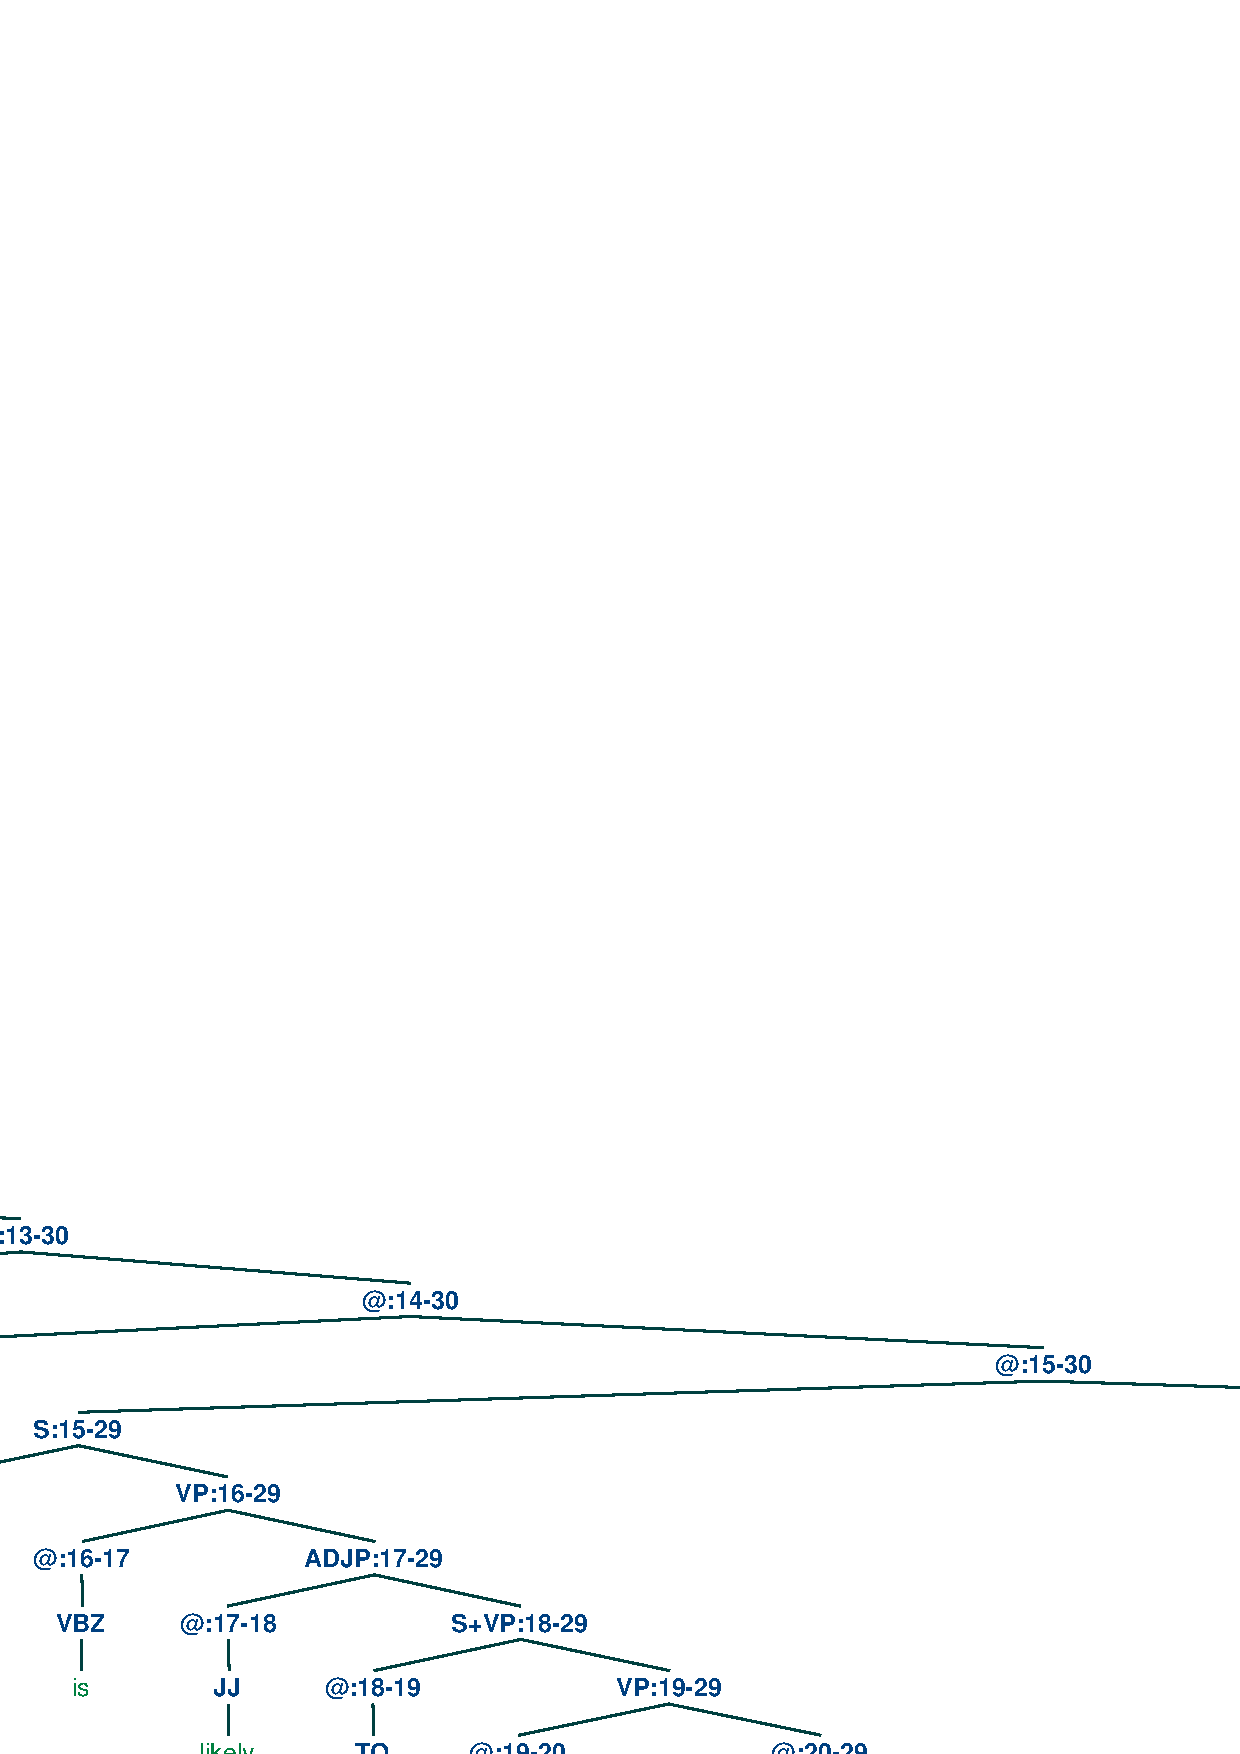
\includegraphics[width=\textwidth]{trees/binary.pdf}
    \caption{Converted to normal form.}
		\label{fig:tree-cnf}
	\end{subfigure}
	\begin{subfigure}{0.9\textwidth}
		\includegraphics[width=\textwidth]{trees/spans.pdf}
    \caption{In normal form with spans.}
		\label{fig:tree-cnf-spans}
	\end{subfigure}
  \caption{Converting a treebank tree (withouth part-of-speech tags).}
  \label{fig:trees}
\end{figure}

% \begin{figure}
% 	\centering
%   \small
%   \begin{subfigure}{0.72\textwidth}
%     \begin{tikzpicture}
%       \input{../figures/trees/simplified.tex}
%     \end{tikzpicture}
%     \caption{Original Penn Treebank tree.}
% 		\label{fig:tree-original}
% 	\end{subfigure}
% 	\begin{subfigure}{0.62\textwidth}
%     \begin{tikzpicture}
% 		  \input{../figures/trees/simplified.tex}
%     \end{tikzpicture}
%     \caption{Function tags and traces removed.}
% 		\label{fig:tree-simplified}
% 	\end{subfigure}
% 	\begin{subfigure}{0.62\textwidth}
%     \begin{tikzpicture}
% 		  \Tree [.S
        [.SBAR [.WHNP What ] [.S+VP [.@ happened ] [.NP Friday ] ] ]
        [.@
          [.VP
            [.@ was ]
            [.NP
              [.NP [.@ the ] [.@ worst ] ]
              [.PP [.@ of ] [.NP [.@ all ] [.@ worlds ] ] ] ] ]
          [.@ . ] ] ]

%     \end{tikzpicture}
%     \caption{Converted to normal form.}
% 		\label{fig:tree-cnf}
% 	\end{subfigure}
% 	\begin{subfigure}{\textwidth}
%     \begin{tikzpicture}
% 		  % \Tree [.S:0-10
%         [.SBAR:0-3
%           [.WHNP:0-1 What ]
%           [.S+VP:1-3 [.$\varnothing$:1-2 happened ] [.NP:2-3 Friday ] ] ]
%         [.$\varnothing$:3-10
%           [.VP:3-9
%             [.$\varnothing$:3-4 was ]
%             [.NP:4-9
%               [.NP:4-6 [.$\varnothing$:4-5 the ] [.$\varnothing$:5-6 worst ] ]
%               [.PP:6-9
%                 [.$\varnothing$:6-7 of ]
%                 [.NP:7-9 [.$\varnothing$:7-8 all ] [.$\varnothing$:8-9 worlds ] ] ] ] ]
%           [.$\varnothing$:9-10 . ] ] ]


\Tree [.S$_0^{10}$
        [.SBAR$_0^3$
           [.WHNP$_0^1$ What ]
          [.S+VP$_1^3$ [.$\varnothing_1^2$ happened ] [.NP$_2^3$ Friday ] ] ]
        [.$\varnothing_3^{10}$
          [.VP$_3^9$
             [.$\varnothing_3^4$ was ]
            [.NP$_4^9$
               [.NP$_4^6$ [.$\varnothing_4^5$ the ] [.$\varnothing_5^6$ worst ] ]
              [.PP$_6^9$
                 [.$\varnothing_6^7$ of ]
                [.NP$_7^9$ [.$\varnothing_7^8$ all ] [.$\varnothing_8^9$ worlds ] ] ] ] ]
          [.$\varnothing_9^{10}$  . ] ] ]

%     \end{tikzpicture}
%     \caption{In normal form with spans.}
% 		\label{fig:tree-cnf-spans}
% 	\end{subfigure}
%   \caption{Converting a treebank tree (withouth part-of-speech tags).}
%   \label{fig:trees}
% \end{figure}

\begin{table}[]
  \small
  \bgroup  % increase vertical space
  \def\arraystretch{1.5}  % increase vertical space
  \begin{tabular}{l|l}
    Labeled spans & Anchored rules \\
    \hline
    (S, 0, 10)     & (S $\to$ SBAR @, 0, 3, 10)  \\
    (SBAR, 0, 3)   & (SBAR $\to$ WHNP S+VP, 0, 1, 3)  \\
    (VP, 1, 3)     & (S+VP $\to$ @ NP, 1, 2, 3)  \\
    $\qquad\vdots$ & $\qquad\vdots$  \\
    (NP, 7, 9)     & (NP $\to$ @ @, 7, 8, 9)  \\
  \end{tabular}
  \caption{Two conceptions of the tree in \ref{fig:tree-cnf-spans}.}
  \label{tab:spans-rules}
  \egroup  % increase vertical space
\end{table}

\section{Neural networks}
Introduce all the neural networks.
\begin{itemize}
  \item Feedforward, RNN, LSTM etc.
  \item We consider these as abstractions denoting certain parametrized functions. A Feedforward network is a function that a vector $\mathbf{x}$ produces an output vector
  \begin{equation*}
    \textsc{FeedForward}_{\theta}( \mathbf{x} ) = \mathbf{y}.
  \end{equation*}
  An $\textsc{RNN}$ is function parametrized by $\theta$ that takes a sequence of vectors $(\mathbf{x_i})_{i=1}^n = ( \mathbf{x}_1, \dots, \mathbf{x}_n )$  and produces a sequence of output vectors:
  \begin{equation*}
    \textsc{rnn}_{\theta}( (\mathbf{x_i})_{i=1}^n ) = ( \mathbf{y}_1, \dots, \mathbf{y}_n ).
  \end{equation*}
  We make use of the notion of a \textit{bidirectional} \textsc{rnn}. This involves applying the \textsc{rnn} function also on the reversed input sequence $rev((\mathbf{x}_1, \dots, \mathbf{x}_n)) \triangleq (\mathbf{x}_n, \dots, \mathbf{x}_1)$, \ie in \textit{backward} direction:
  \begin{align*}
    \textsc{rnn}_{\theta}^B( (\mathbf{x_i})_{i=1}^n )
      &= rev(\textsc{rnn}_{\theta}(rev((\mathbf{x_i})_{i=1}^n))) \\
      &= rev(\textsc{rnn}_{\theta}(\mathbf{x}_n, \dots, \mathbf{x}_1) \\
      &= rev( \mathbf{y}_n, \dots, \mathbf{y}_1 ) \\
      &= ( \mathbf{y}_1, \dots, \mathbf{y}_n ) \\
  \end{align*}
  For convenience we will refer to the regular, \textit{forward}, \textsc{rnn} as $\textsc{rnn}^F$. To stress the difference between the different outputs obtained from the two directions, we will denote the output vectors obtained in the regular, forward, direction with $\mathbf{f}_i$ and the vectors obtained in the backward direction with $\mathbf{b}_i$:
  \begin{align*}
    \textsc{rnn}_{\theta}^B( (\mathbf{x_i})_{i=1}^n ) &= ( \mathbf{b}_1, \dots, \mathbf{b}_n ) \\
    \textsc{rnn}_{\theta}^F( (\mathbf{x_i})_{i=1}^n ) &= ( \mathbf{f}_1, \dots, \mathbf{f}_n ).
  \end{align*}
  An \textsc{lstm} is a particular way to construct the \textsc{rnn} function.
  \item Write down the equations for the Feedforward network, and maybe, maybe, maybe write down the equations for the LSTM.
  \item (Minibatch) SGD optimization.
\end{itemize}

\section{Language models}
\begin{itemize}
  \item Briefly mention some typical approaches for langugage modelling: count based n-gram with smoothing \citep{chen1999empirical,kneser1995improved}, neural n-gram \citep{bengio2003neural} and recurrent neural network \citep{mikolov2010recurrent}. Also mention some (early) syntactic approaches: count-based \citep{chelba2000structured,pauls2012treelets}, neural \citep{emami2005neural}, and top-down parsing related \citep{Roark2001}.
  \item Explain the metric perplexity.
  \item Briefly mentions some typical datasets and some benchmarks (dataset, perplexity, number of parameters, training time).
  \item Mention some downsides of the perplexity metric: conflating different sources of succes in next-word prediction (simple collocations, semantics, syntax).
  \item Note that there exists some alternatives to perplexity: adversarial evaluation \citep{Smith2012:adversarial}, subject-verb agreement \citep{Linzen+2016:LSTM-syntax} and grammatical acceptability judgments \citep{Linzen+2018:targeted}.
\end{itemize}
